\documentclass[portrait,final,a0paper,fontscale=0.277]{baposter}

\usepackage{calc}
\usepackage{graphicx}
\usepackage{amsmath}
\usepackage{amssymb}
\usepackage{relsize}
\usepackage{multirow}
\usepackage{rotating}
\usepackage{bm}
\usepackage{url}

\usepackage{graphicx}
\usepackage{multicol}

\usepackage[]{algorithm2e}
\SetKwComment{Comment}{$\triangleright$\ }{}



%\usepackage{times}
%\usepackage{helvet}
%\usepackage{bookman}
\usepackage{palatino}

\newcommand{\captionfont}{\footnotesize}

\graphicspath{{images/}{../images/}}
\usetikzlibrary{calc}

\newcommand{\SET}[1]  {\ensuremath{\mathcal{#1}}}
\newcommand{\MAT}[1]  {\ensuremath{\boldsymbol{#1}}}
\newcommand{\VEC}[1]  {\ensuremath{\boldsymbol{#1}}}
\newcommand{\Video}{\SET{V}}
\newcommand{\video}{\VEC{f}}
\newcommand{\track}{x}
\newcommand{\Track}{\SET T}
\newcommand{\LMs}{\SET L}
\newcommand{\lm}{l}
\newcommand{\PosE}{\SET P}
\newcommand{\posE}{\VEC p}
\newcommand{\negE}{\VEC n}
\newcommand{\NegE}{\SET N}
\newcommand{\Occluded}{\SET O}
\newcommand{\occluded}{o}

%%%%%%%%%%%%%%%%%%%%%%%%%%%%%%%%%%%%%%%%%%%%%%%%%%%%%%%%%%%%%%%%%%%%%%%%%%%%%%%%
%%%% Some math symbols used in the text
%%%%%%%%%%%%%%%%%%%%%%%%%%%%%%%%%%%%%%%%%%%%%%%%%%%%%%%%%%%%%%%%%%%%%%%%%%%%%%%%

%%%%%%%%%%%%%%%%%%%%%%%%%%%%%%%%%%%%%%%%%%%%%%%%%%%%%%%%%%%%%%%%%%%%%%%%%%%%%%%%
% Multicol Settings
%%%%%%%%%%%%%%%%%%%%%%%%%%%%%%%%%%%%%%%%%%%%%%%%%%%%%%%%%%%%%%%%%%%%%%%%%%%%%%%%
\setlength{\columnsep}{1.5em}
\setlength{\columnseprule}{0mm}

%%%%%%%%%%%%%%%%%%%%%%%%%%%%%%%%%%%%%%%%%%%%%%%%%%%%%%%%%%%%%%%%%%%%%%%%%%%%%%%%
% Save space in lists. Use this after the opening of the list
%%%%%%%%%%%%%%%%%%%%%%%%%%%%%%%%%%%%%%%%%%%%%%%%%%%%%%%%%%%%%%%%%%%%%%%%%%%%%%%%
\newcommand{\compresslist}{%
\setlength{\itemsep}{1pt}%
\setlength{\parskip}{0pt}%
\setlength{\parsep}{0pt}%
}

%%%%%%%%%%%%%%%%%%%%%%%%%%%%%%%%%%%%%%%%%%%%%%%%%%%%%%%%%%%%%%%%%%%%%%%%%%%%%%
%%% Begin of Document
%%%%%%%%%%%%%%%%%%%%%%%%%%%%%%%%%%%%%%%%%%%%%%%%%%%%%%%%%%%%%%%%%%%%%%%%%%%%%%

\begin{document}

%%%%%%%%%%%%%%%%%%%%%%%%%%%%%%%%%%%%%%%%%%%%%%%%%%%%%%%%%%%%%%%%%%%%%%%%%%%%%%
%%% Here starts the poster
%%%---------------------------------------------------------------------------
%%% Format it to your taste with the options
%%%%%%%%%%%%%%%%%%%%%%%%%%%%%%%%%%%%%%%%%%%%%%%%%%%%%%%%%%%%%%%%%%%%%%%%%%%%%%
% Define some colors

%\definecolor{lightblue}{cmyk}{0.83,0.24,0,0.12}
\definecolor{lightblue}{rgb}{0.145,0.6666,1}

% Draw a video
\newlength{\FSZ}
\newcommand{\drawvideo}[3]{% [0 0.25 0.5 0.75 1 1.25 1.5]
   \noindent\pgfmathsetlength{\FSZ}{\linewidth/#2}
   \begin{tikzpicture}[outer sep=0pt,inner sep=0pt,x=\FSZ,y=\FSZ]
   \draw[color=lightblue!50!black] (0,0) node[outer sep=0pt,inner sep=0pt,text width=\linewidth,minimum height=0] (video) {\noindent#3};
   \path [fill=lightblue!50!black,line width=0pt] 
     (video.north west) rectangle ([yshift=\FSZ] video.north east) 
    \foreach \x in {1,2,...,#2} {
      {[rounded corners=0.6] ($(video.north west)+(-0.7,0.8)+(\x,0)$) rectangle +(0.4,-0.6)}
    }
;
   \path [fill=lightblue!50!black,line width=0pt] 
     ([yshift=-1\FSZ] video.south west) rectangle (video.south east) 
    \foreach \x in {1,2,...,#2} {
      {[rounded corners=0.6] ($(video.south west)+(-0.7,-0.2)+(\x,0)$) rectangle +(0.4,-0.6)}
    }
;


   \foreach \x in {1,...,#1} {
     \draw[color=lightblue!50!black] ([xshift=\x\linewidth/#1] video.north west) -- ([xshift=\x\linewidth/#1] video.south west);
   }
   \foreach \x in {0,#1} {
     \draw[color=lightblue!50!black] ([xshift=\x\linewidth/#1,yshift=1\FSZ] video.north west) -- ([xshift=\x\linewidth/#1,yshift=-1\FSZ] video.south west);
   }
   \end{tikzpicture}
}

\hyphenation{resolution occlusions}
%%
\begin{poster}%
  % Poster Options
  {
  % Show grid to help with alignment
  grid=false,
  % Column spacing
  colspacing=1em,
  % Color style
  bgColorOne=white,
  bgColorTwo=white,
  borderColor=lightblue,
  %headerColorOne=black,
  headerColorOne=lightblue,
  headerColorTwo=lightblue,
  headerFontColor=white,
  boxColorOne=white,
  boxColorTwo=lightblue,
  % Format of textbox
%  textborder=roundedleft,
  textborder=rounded,
  % Format of text header
  eyecatcher=true,
  headerborder=closed,
  headerheight=0.1\textheight,
%  textfont=\sc, An example of changing the text font
  %headershape=roundedright,
  headershape=rounded,
  %headershade=shadelr,
  headerfont=\Large\bf\textsc, %Sans Serif
  textfont={\setlength{\parindent}{1.5em}},
  boxshade=plain,
%  background=shade-tb,
  background=plain,
  linewidth=2pt
  }
  % Eye Catcher
  {} 
  % Title
  {PLC Factory: Automating routine tasks in large-scale PLC software development \vspace{0.2em}}
  % Authors
  {G. Ulm, F. Bellorini, D. Brodrick, R. Fernandes,\\ N. Levchenko, D. Piso Fernandez}
  % University logo
  {% The makebox allows the title to flow into the logo, this is a hack because of the L shaped logo.
    
\includegraphics[height=9.0em]{logo/ESS}
  }
  
  
  
  
  
  
  



%%%%%%%%%%%%%%%%%%%%%%%%%%%%%%%%%%%%%%%%%%%%%%%%%%%%%%%%%%%%%%%%%%%%%%%%%%%%%%
%%% Now define the boxes that make up the poster
%%%---------------------------------------------------------------------------
%%% Each box has a name and can be placed absolutely or relatively.
%%% The only inconvenience is that you can only specify a relative position 
%%% towards an already declared box. So if you have a box attached to the 
%%% bottom, one to the top and a third one which should be in between, you 
%%% have to specify the top and bottom boxes before you specify the middle 
%%% box.
%%%%%%%%%%%%%%%%%%%%%%%%%%%%%%%%%%%%%%%%%%%%%%%%%%%%%%%%%%%%%%%%%%%%%%%%%%%%%%
    %
    % A coloured circle useful as a bullet with an adjustably strong filling
    \newcommand{\colouredcircle}{%
      \tikz{\useasboundingbox (-0.2em,-0.32em) rectangle(0.2em,0.32em); \draw[draw=black,fill=lightblue,line width=0.03em] (0,0) circle(0.18em);}}


%%%%%%%%%%%%%%%%%%%%%%%%%%%%%%%%%%%%%%%%%%%%%%%%%%%%%%%%%%%%%%%%%%%%%%%%%%%%%%
  \headerbox{Problem}{name=problem,column=0,row=0}{
%%%%%%%%%%%%%%%%%%%%%%%%%%%%%%%%%%%%%%%%%%%%%%%%%%%%%%%%%%%%%%%%%%%%%%%%%%%%%%
\noindent
The European Spallation Source ERIC~(ESS) in Lund, Sweden, is building large-scale infrastructure that is projected to include hundreds of programmable logic controllers (PLCs). The problem is:
   \begin{enumerate}\compresslist
      \item PLCs directly control hardware, thus programming errors can have serious consequences
      \item Programming PLCs is repetitive and error-prone 
      \item Some repetitions are not trivial to automate
   \end{enumerate}
   \vspace{0.3em}
 }
 
 
 

%%%%%%%%%%%%%%%%%%%%%%%%%%%%%%%%%%%%%%%%%%%%%%%%%%%%%%%%%%%%%%%%%%%%%%%%%%%%%%
  \headerbox{Contributions}{name=contribution,column=0,below=problem}{
%%%%%%%%%%%%%%%%%%%%%%%%%%%%%%%%%%%%%%%%%%%%%%%%%%%%%%%%%%%%%%%%%%%%%%%%%%%%%%
\noindent
PLC Factory is an application for automating repetitive tasks associated with PLC programming. It relies on an in-house configuration database, CCDB, which stores information for each device instance and device type. PLC Factory is a template-based substitution engine that performs the following tasks:

\begin{enumerate}

\item direct substitution, i.e.\ for a given device~$d$, use property~$p$ as specified in the corresponding CCDB entry for $d$

\item identification of shared properties between devices, in order to remove redundancies in CCDB

\item automatic counters management for specifying PLC memory address offsets in EPICS database records

\end{enumerate}

   \vspace{0.3em}
  }

%%%%%%%%%%%%%%%%%%%%%%%%%%%%%%%%%%%%%%%%%%%%%%%%%%%%%%%%%%%%%%%%%%%%%%%%%%%%%%
\headerbox{Solution}{name=results,column=1,span=2,row=0}{
  %%%%%%%%%%%%%%%%%%%%%%%%%%%%%%%%%%%%%%%%%%%%%%%%%%%%%%%%%%%%%%%%%%%%%%%%%%%%%%
\begin{multicols}{2}
\noindent
The substitutions outlined in \emph{Contributions} remove most if not all of the repetitions of large-scale PLC software development. We highlight four aspects of PLC Factory.

\paragraph{Dependency Trees}
CCDB describes dependency relationships between devices; a \emph{dependency tree} explicitly models those. In the example below, $r$ is the root device and controls the devices $u_1$ and $u_2$, of which the former controls $v_{11}$ and $v_{12}$, and the latter $v_{21}$. Trees can be arbitrarily deep.

\vspace{5mm}
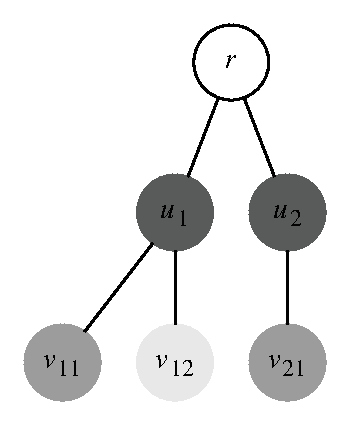
\includegraphics[width=0.50\linewidth]{figures/deviceTreeCropped.eps}


\paragraph{Template Files}
Template files are text files with a fixed structure. PLC Factory consumes template files for creating EPICS database records files and SCL code blocks for TIA Portal. Device types may have template files with particular IDs attached to it in CCDB. PLC Factory \emph{dynamically} replaces fields within a template file. A simplified example is the substitution of a field \texttt{DEVICE\_NAME} by the concrete name of a device that is an instance of the device type this template is associated with.



\paragraph{Substitution Engine}
Pseudo-code of the core of the substitution engine is given below. The operator $\oplus$ is a shorthand for processing template files. It is applied to a device instance $x$ and a specific template. Templates are retrieved by a function $t$ that takes as its input a template ID and the device type of $x$, which is determined by the function $d$ applied to device $x$. Thus, the resulting operation is $x \oplus t(\mathit{id}, d(x))$.

\columnbreak

\noindent
In addition, we define the header file $h(\mathit{id}, d(r))$ as well as the footer file $f(\mathit{id}, d(r))$.

\vspace{5mm}

\begin{minipage}[t]{0.8\linewidth}
   \vspace{-2ex}
 \label{alg:algo}
 \KwData{CCDB, root device $r$, template ID $id$}
 \KwResult{list \emph{out} containing text for post-processing}
\Begin{
 $\mathit{out} \leftarrow  \varnothing$  \Comment*[f]{collected output}  \\
 $\mathit{ds} \leftarrow r$   \Comment*[f]{list of devices} \\
 \While{ ds \emph{not $\varnothing$ } }{
  $d \leftarrow$  $ds$.pop() \\
  $cs \leftarrow $ $d$.controls()  \Comment*[f]{CCDB lookup}  \\
  \While{ cs \emph{not} $\varnothing$  }{
    $c \leftarrow$ $\mathit{cs}$.pop() \\
    \If{  $ t(\mathit{id}, d(c)) \in $ CCDB} { 
           $\mathit{out} \leftarrow \mathit{out} + c \oplus  t(\mathit{id}, d(c))  $  \\
           $\mathit{cs}' \leftarrow c.$controls() \\
           $\mathit{ds} \leftarrow \mathit{ds} + \mathit{cs}'$ \\
   }
  }  
 }
$\mathit{out} \leftarrow r \oplus  h(\mathit{id}, d(r))    + \mathit{out} + r \oplus f(\mathit{id}, d(r))   $   \\
 }   
\end{minipage}


\paragraph{PLCF$^\sharp$}
\noindent
PLCF$^\sharp$ is an embedded domain-specific language for flexible substitutions. It solves two problems: resolving shared property values and manual memory management. For the former, consider the expression \texttt{[PLCF\# \textasciicircum(Offset) + 1]}. Here, PLC Factory looks up the property \texttt{Offset} by traversing the device tree upwards. For the latter case, consider the expression \texttt{[PLCF\# \textasciicircum(Offset) + Counter1]}. In this example, counter variables automate assigning memory addresses. The user only has to specify which counter should be incremented. A large skeleton file for TIA Portal may contain hundreds of memory locations. PLC Factory completely automates their definition and ensures there are no overlaps.

\end{multicols}





}
%%%%%%%%%%%%%%%%%%%%%%%%%%%%%%%%%%%%%%%%%%%%%%%%%%%%%%%%%%%%%%%%%%%%%%%%%%%%%%
  \headerbox{References}{name=references,column=0,above=bottom}{
%%%%%%%%%%%%%%%%%%%%%%%%%%%%%%%%%%%%%%%%%%%%%%%%%%%%%%%%%%%%%%%%%%%%%%%%%%%%%%
    \smaller
    \bibliographystyle{ieee}
    \renewcommand{\section}[2]{\vskip 0.05em}
      \begin{thebibliography}{1}\itemsep=-0.01em
      \setlength{\baselineskip}{0.4em}
      
      \bibitem{Borrowman} Borrowman, A. J., \& Taylor, P. (2016, July). Can your software engineer program your PLC?. In SPIE Astronomical Telescopes+ Instrumentation (pp. 99131S-99131S). International Society for Optics and Photonics.

\bibitem{CasasCubillos2002} Casas-Cubillos, J., Gomes, P., Gayet, P., Varas, F. J., Sicard, C. H., \& Pezzetti, M. (2002). Application of object-based industrial controls for cryogenics (No. CERN-LHC-2002-007-IAS).

\bibitem{Cockrell1992} Cockrell, L., \& Sander, T. M. (1992). Selecting a man/machine interface for a PLC-based process control system. IEEE transactions on industry applications, 28(4), 945-953.

\bibitem{EPICS} Dalesio, L. R., Kraimer, M. R., \& Kozubal, A. J. (1991, November). EPICS architecture. In ICALEPCS (Vol. 91, pp. 92-15).

%\bibitem{CCDB-ESS} Fernandes et al., forthcoming 2016

\bibitem{CCDB-CERN} Zaharieva, Z., Peryt, M., \& Martin Marquez, M. (2011, October). Database foundation for the configuration management of the CERN accelerator controls systems. In Conf. Proc. (Vol. 111010,  No. CERN-ATS-2011-206, p. MOMAU004).




      

      
      
      \end{thebibliography}
   \vspace{0.3em}
  }
  
%%%%%%%%%%%%%%%%%%%%%%%%%%%%%%%%%%%%%%%%%%%%%%%%%%%%%%%%%%%%%%%%%%%%%%%%%%%%%%
  \headerbox{Future Work}{name=background model,column=1,below=results}{
%%%%%%%%%%%%%%%%%%%%%%%%%%%%%%%%%%%%%%%%%%%%%%%%%%%%%%%%%%%%%%%%%%%%%%%%%%%%%%
\noindent
PLC Factory is a command-line application. We intend to turn it into the backbone of a web-based GUI-driven application. Further, we consider extending PLC Factory by adding an exporter to automatically generate operator interfaces (OPIs). PLC Factory can be easily tailored to use other database backends as well, so adding interfaces would be another suitable next step. However, PLC Factory does not rely on domain knowledge. Due to its generic approach to template processing it could be used in many other domains as well, as it is a universal template-based substitution engine.



  }
  
  
%%%%%%%%%%%%%%%%%%%%%%%%%%%%%%%%%%%%%%%%%%%%%%%%%%%%%%%%%%%%%%%%%%%%%%%%%%%%%%
\headerbox{Source Code}{name=speed,column=2,row=0,below=results,bottomaligned=background model}{
  %%%%%%%%%%%%%%%%%%%%%%%%%%%%%%%%%%%%%%%%%%%%%%%%%%%%%%%%%%%%%%%%%%%%%%%%%%%%%%
\noindent
PLC Factory has been written in Python 2.7. The application is used in production and is actively maintained by ESS. We made the source code available under the third version of the GNU General Public License (GNU GPLv3). The project repository is:\\ \\
 \texttt{https://bitbucket.org/\linebreak europeanspallationsource/ \linebreak ics\_plc\_factory}.

  }




%%%%%%%%%%%%%%%%%%%%%%%%%%%%%%%%%%%%%%%%%%%%%%%%%%%%%%%%%%%%%%%%%%%%%%%%%%%%%%
  \headerbox{Results}{name=method,column=0,below=contribution,above=references}{
%%%%%%%%%%%%%%%%%%%%%%%%%%%%%%%%%%%%%%%%%%%%%%%%%%%%%%%%%%%%%%%%%%%%%%%%%%%%%%
  \noindent
The time complexity of PLC Factory is $O(n)$, where $n$ the number of devices. On a 2011 MacBook Air (1.8 GHz), PLC Factory processes three different template IDs for a tree with 40 devices in 7 seconds. Manually creating those files would take many hours.

  
  
  }

\end{poster}

\end{document}

